\documentclass[conference]{IEEEtran}

\usepackage{amsmath}
\usepackage{graphicx}
\usepackage{subfig}
\usepackage{paralist}

\providecommand{\e}[1]{\ensuremath{\times 10^{#1}}}

% correct bad hyphenation here
\hyphenation{op-tical net-works semi-conduc-tor}

\begin{document}

\title{Predicting Reciprocity in Social Networks}

\author{\IEEEauthorblockN{Anonymous}
\IEEEauthorblockA{Anonymous Department\\
Anonymous Institution \\
Anonymous Location \\
anon@whoare.you}
\and
\IEEEauthorblockN{Anonymous}
\IEEEauthorblockA{Anonymous Department\\
Anonymous Institution \\
Anonymous Location \\
anon@whoare.you}
\and
\IEEEauthorblockN{Anonymous}
\IEEEauthorblockA{Anonymous Department\\
Anonymous Institution \\
Anonymous Location \\
anon@whoare.you}}

% make the title area
\maketitle

\begin{abstract}
%\boldmath
In this paper we investigate methods of predicting reciprocity in social networks, and use machine learning (and regression?) to determine good indicators of reciprocity. Using the Twitter @ message graph, we find that XXX and XXX perform well, while XXX and XXX do not, despite the fact that they are good link prediction heuristics.
\end{abstract}

% no keywords

% For peer review papers, you can put extra information on the cover
% page as needed:
% \ifCLASSOPTIONpeerreview
% \begin{center} \bfseries EDICS Category: 3-BBND \end{center}
% \fi
%
% For peerreview papers, this IEEEtran command inserts a page break and
% creates the second title. It will be ignored for other modes.
\IEEEpeerreviewmaketitle

\section{Introduction}
Reciprocity prediction and link prediction are inherently different problems - while link prediction is about predicting the occurence of rare events, reciprocity prediction predicts the "balance", or directions of an edge.

\subsection{Related work}
Tyler and Tang showed that reciprocity 
http://www.hpl.hp.com/research/idl/papers/rhythms/ECSCWFinal.pdf
To be written.

\subsection{Twitter as a domain to analyze}
Twitter is a good domain to explore the superposition of the reciprocated and unreciprocated networks. The reciprocated network consists of mainly mutual interactions between friends or people in the same social circle, while the unreciprocated network consists of interactions between individuals in different social circles. We can also relate these types of interactions to the concept of status - where people with similar status participate in reciprocal interactions (e.g. messages between friends), while those with dissimilar status participate in unreciprocal interactions (e.g. messages from fans to celebrities).

\subsection{Problem definition}
The input to our prediction problem is a graph $G=(V,E)$ and a node pair $\{v,w\}$, where $v,w \in V$ but all edges between $v$ and $w$ removed. Our task is to predict the direction of edges between $v$ and $w$.

Reciprocity prediction on this graph can be defined in two ways. In the first, given that at least one edge exists between $v$ and $w$, decide whether both $(v,w)$ and $(w,v)$ exist (bidirected/symmetric), or only one of $(v,w)$, $(w,v)$ exists (asymmetry). In the second, given an edge $(v,w)$, decide whether $(w,v)$ exists.

\subsection{Notation}

We subsequently consider the subgraphs of the form $G_n = (V_n, E_n)$, where $V_n = \{v~|~v \in V, v \text{ sent } \ge n \text{ messages}\}$ and $E_n = \{e=(v,w)~|~e \in E,~v \text{ and } w \in V_n\}$.

Also define \(v \xrightarrow{k} w$, which means $v$ sent $w$ $k$ messages. From this definition we can formalize reciprocity in terms of $k$. We define an edge $(v,w)$ to be reciprocated if $v \xrightarrow{k} w$ and $w \xrightarrow{k} v$, and unreciprocated if $v \xrightarrow{k} w$ and $w \xrightarrow{0} v$.

Let the set of reciprocated edges be \(E_k^r = \{ (v,w) : v \xrightarrow{k} w \text{ and } w \xrightarrow{k} v \} \), and the set of unreciprocated edges be \(E_k^u = \{ (v,w) : v \xrightarrow{k} w\} \).

Let $\deg^-(v)$ and $\deg^+(v)$ be the indegree and outdegree of node $v$ respectively, $\operatorname{msg}^-(v)$ and $\operatorname{msg}^+(v)$ be the messages received and sent by a node $v$, and $\Gamma^-(v) = \{w| (w,v) \in E\}$, or the set of people who send messages to $v$.

\section{Dataset description}
The sample dataset consisted of the directed @ message graph $G=(V,E)$ of the Twitter network from (TIME) to (TIME). 12,795,683 unique users ($|V|$) sent a total of 819,305,776 messages, with 156,868,257 unique directed interactions ($|E|$) taking place between users during this time.

In $G_{1000}$, $|E^r_{10}| = 797,342$, $|E^u_{10}| = 349,258$.

\section{Methods for Reciprocity Prediction}
Intuitively, features and measure whether $v$ and $w$ have similar status or a similar social circle, and each is potentially useful in predicting reciprocation. This section presents a survey of various methods that can be used in predicting reciprocity in networks. Each method assigns a value $\operatorname{val}(v,w)$ to a node pair $\{v,w\}$. Given values corresponding to all node pairs in question, we can then choose threshold values or ranges where we predict reciprocity, and non-reciprocity otherwise.

For each property, we picked a single value $v^\star$ for which we predict every edge with value lower than $v^\star$ is unreciprocated and reciprocated otherwise, or vice versa, to maximize prediction accuracy. Intuitively, we expect that larger values of each property correspond to a stronger indication of reciprocity. For example, a high mutual neighbor count for the nodes $v$ and $w$ could strongly indicate the existence of a reciprocated link between them.

We considered 3 different mechanisms of prediction: 
\begin{enumerate}
\item SYM (predicting symmetry), where we predict whether an edge is bidirectional or asymmetric after removing all information about the edge in question but using existing information about $v$ and $w$, 
\item REV (predicting a reverse edge), where we predict whether a reverse edge exists given that the forward edge $(v,w)$ exists using information about $v$ and $w$, and finally 
\item REVW (predicting a reverse edge using only $w$), where we predict whether a reverse edge exists given that $(v,w)$ exists, but only using information about $w$ in making that prediction.
\item REVV (predicting a reverse edge using only $v$), where we predict whether a reverse edge exists given that $(v,w)$ exists, but only using information about $v$ in making that prediction.
\end{enumerate}

\subsection{Degree/message-based prediction features}
It seems intuitive that the relative indegree or outdegree of nodes would indicate whether a pair of nodes are in a one-sided or two-sided relationship. If both have a similar indegree, this might indicate that they are at a similar social status in the network. In contrast, a disproportionate indegree would indicate that one might be a celebrity and the other an average Joe, thus it would be unlikely that the relationship between them is reciprocated.

\emph{Indegree and outdegree ratio} both measure the ratio of outdegrees or indegrees of two nodes, and $\operatorname{val}(v,w) = \deg^-(v)/\deg^-(w)$ or $\deg^+(v)/\deg^+(w)$ respectively.

\emph{Inmessage and outmessage ratio} are similar, but instead also take into account the total number of messages that a node receives or sends, rather than the unique nodes that a node sends messages to or receives messages from.

\emph{Incoming message/indegree ratio and outgoing message/outdegree ratio} compares the ratio of two nodes' incoming message to indegree ratio or outgoing message to outdegree ratio. People with a high incoming message to indegree ratio might characterize people who have a small group of friends with which they exchange lots of messages, while those with a low incoming message to indegree ratio might characterize highly connected (and thus high-status) people in a network (as the messages they receive is "spread" over many more users).

\emph{Outdegree/indegree ratio} is a heuristic that attempts to characterize the messaging activity of a single node - a celebrity might have high outdegree/indegree ratio because she receive many messages from many followers but herself sends relatively few messages. We then characterize the ratio of the outdegree/indegree ratio of two nodes, or $\operatorname{val}(v,w) = \frac{\deg^+(v)}{\deg^-(v)} / \frac{\deg^+(w)}{\deg^-(w)}$.

\subsection{Link prediction features}
It is not intuitive whether methods that work well for link prediction would work well in reciprocity; while link prediction asks whether an edge could exist between two nodes, reciprocity prediction asks whether a known edge is bidirectional.

\emph{Jaccard's coefficient} calculates the similarity between two sets by taking the ratio of the cardinality of their intersection and their union. $\operatorname{val}(v,w) = \frac{|\Gamma^-(v) \cap \Gamma^-(w)|}{|\Gamma^-(v) \cup \Gamma^-(w)|}$.

\emph{Adamic and Adar} \cite{Adamic:2003ud}, defined the similarity between web sites $v,w$ to be $ \sum_{\{x|v,w \text{ share feature }x\}} \frac{1}{\log{\text{frequency}(x)}} $, and we similarly define $\operatorname{val}(v,w)$ to be \[ \sum_{\{x|x \in \Gamma^-(v) \cap \Gamma^-(w)\}} \frac{1}{\log{\deg^-(x)}} .\]

\emph{Preferential attachment} is another popular heuristic in modeling network growth, where the probability that an edge forms with a specific node is proportional to its existing indegree. Here, $\operatorname{val}(v,w) = \deg^-(v)\cdot \deg^-(w)$.

\emph{2 step paths (ratio)} is a simplification of what Katz \cite{Katz:1953un} developed as a measure of status by calculating the number of paths between two nodes. In this study, we only consider paths of length 2, and $\operatorname{val}(v,w) = \sum_{i=1}^2 \beta^i|\operatorname{paths}^i(v,w)|$, where $\beta$ is an arbitary damping constant, and $\operatorname{paths}^i(v,w)$ is the set of paths from $v$ to $w$ of length $i$. The 2 step paths ratio is simply the ratio of number of two step paths from $v$ to $w$ to that from $w$ to $v$. TODO I can also calculate that in the case where you predict a reverse edge, you use the path from $v$ to $w$ in your calculation, thus adding a single on-step path to the calculation.

\begin{table}[!t]
\renewcommand{\arraystretch}{1.3}
\caption{Reciprocity Prediction Features}
\label{table_recmethods}
\centering
\begin{tabular}{|c||c|}
\hline
\bf{Feature} & $\mathbf{val}(v)$ or $\mathbf{val}(v,w)$\\
\hline
Indegree or outdegree & $\deg^-(v)$ or $\deg^+(v)$ \\
Incoming or outgoing messages & $\operatorname{msg}^-(v)$ or $\operatorname{msg}^+(v)$ \\
Message-degree (in or out) & $\frac{\operatorname{msg}^-(v)}{\deg^-(v)}$ or $\frac{\operatorname{msg}^+(v)}{\deg^+(v)}$ \\
Outdegree-indegree & $\frac{\deg^+(v)}{\deg^-(v)}$ \\
\hline
\hline
Indegree ratio & $\deg^-(v) / \deg^-(w)$ \\
Outdegree ratio & $\deg^+(v) / \deg^+(w)$ \\
\hline
Incoming message ratio & $\operatorname{msg}^-(v) / \operatorname{msg}^-(w)$ \\
Outgoing message ratio & $\operatorname{msg}^+(v) / \operatorname{msg}^+(w)$ \\
\hline
Incoming message-indegree ratio & $\frac{\operatorname{msg}^-(v)}{\deg^-(v)} / \frac{\operatorname{msg}^-(w)}{\deg^-(w)}$ \\
Outgoing message-indegree ratio & $\frac{\operatorname{msg}^+(v)}{\deg^+(v)} / \frac{\operatorname{msg}^+(w)}{\deg^+(w)}$ \\
\hline
Outdegree-indegree ratio & $\frac{\deg^+(v)}{\deg^-(v)} / \frac{\deg^+(w)}{\deg^-(w)} $ \\
\hline
\hline
Mutual neighbors (in) & $|\Gamma^-(v) \cap \Gamma^-(w)|$ \\
Mutual neighbors (out) & $|\Gamma^+(v) \cap \Gamma^+(w)|$ \\
\hline
Jaccard's coefficient (in) & $\frac{|\Gamma^-(v) \cap \Gamma^-(w)|}{|\Gamma^-(v) \cup \Gamma^-(w)}$ \\
Jaccard's coefficient (out) & $\frac{|\Gamma^+(v) \cap \Gamma^+(w)|}{|\Gamma^+(v) \cup \Gamma^+(w)}$ \\
\hline
Adamic/Adar & $\sum_{\{x|x \in \Gamma^-(v) \cap \Gamma^-(w)\}} \frac{1}{\log{\deg^-(x)}}$ \\
\hline
Preferential attachment ($v$ to $w$) & $\deg^+(v)\cdot \deg^+(w)$ \\
Preferential Attachment ($w$ to $v$) & $\deg^-(v)\cdot \deg^-(w)$ \\
\hline
Two-step paths ($v$ to $w$) & $ |\operatorname{paths}^2(v,w)|$ \\
Two-step paths ($w$ to $v$) & $ |\operatorname{paths}^2(w,v)|$ \\
\hline
Two-step paths ratio & $\frac{|\operatorname{paths}^2(v,w)|}{|\operatorname{paths}^2(w,v)|}$ \\
% $\frac{\sum_{i=1}^2 \beta^i|\operatorname{paths}^i(v,w)|}{\sum_{i=1}^2 \beta^i|\operatorname{paths}^i(w,v)|}$ Did badly
\hline
\end{tabular}
\end{table}

\section{Results and Discussion}

\subsection{Individual properties}
To calculate the accuracy of the individual heuristics, we calculated the values obtained for each method on a subset of $E_{10}^r \cup E_{10}^u$ of the graph $G_{1000}$, where equal numbers of edges were taken from the two sets of reciprocated and unreciprocated edges. The baseline accuracy is 0.500, since you would achieve this by simply predicting that all edges were of one type.

We then picked a threshold value $\operatorname{val}_{OPT}$ to optimize prediction accuracy, where we would predict reciprocity above the threshold, and non-reciprocity otherwise (or vice versa). Table \ref{table_recresults_indiv} summarizes the performance of each heuristic on the subgraph $G_{1000}, k=10$, while table \ref{table_recresults_indeg} summarizes the different mechanisms of prediction for a single heuristic. 

\subsubsection{Comparison of mechanisms of prediction}

In table \ref{table_recresults_indeg}, SYM$^+$ refers to the prediction mechanism where we aim to predict symmetry and predict all edges with values \emph{above} $val_{OPT}$ to be reciprocated, and REV$^-$ refers to the mechanism where we aim to predict whether a reverse edge $(w,v)$ exists given $(v,w)$ and predict all edges with values \emph{below} $val_{OPT}$ to be reciprocated. 

We observe slightly higher accuracy for the REV task than SYM, as REV is ``easier" than SYM since you know more information about the edge $(v,w)$. Surprisingly, REVW performs even better TODO Why? We do notice that in all cases you want to predict that the top 40\% of values as being reciprocated. 

Note that SYM$^-$, REV$^-$ and REVW$^+$ did so poorly that simply predicting that everything was reciprocated (or unreciprocated) would do better.

\subsubsection{Comparison of methods of prediction}
On the whole, outdegree-indegree ratio and the two-step paths ratio are the best indicators of reciprocity.

\begin{table}[!t]
\renewcommand{\arraystretch}{1.3}
\caption{Indegree performance - different methods}
\label{table_recresults_indeg}
\centering
\begin{tabular}{|c||c|c|}
\hline
\bf{Mechanism} & $\mathbf{val}_{OPT}$ (Percentile) & \bf{Accuracy} \\
\hline
SYM$^+$ & 0.256 (40) & 0.702 \\
SYM$^-$ & - & - \\
REV$^+$ & 0.261 (40) & 0.705 \\
REV$^-$ & - & - \\
REVW$^+$ & - & - \\
REVW$^-$ & 74 (61) & 0.731 \\
\hline
\end{tabular}
\end{table}

\begin{table}[!t]
\renewcommand{\arraystretch}{1.3}
\caption{Reciprocity Prediction Method Performance: Individual (REV)}
\label{table_recresults_indiv}
\centering
\begin{tabular}{|c||c|c|}
\hline
\bf{Method} & $\mathbf{val}_{OPT}$ (Percentile) & \bf{Accuracy} \\
\hline
Indegree ratio & 0.261 (40) & 0.705 \\
Outdegree ratio & 0.398 (35) & 0.579 \\
\hline
Incoming message ratio & 0.202 (42) & 0.721 \\
Outgoing message ratio & 0.681 (61) & 0.507 \\
\hline
Incoming message-indegree ratio & 0.462 (38) & 0.551 \\
Outgoing message-outdegree ratio & 0.477 (33) & 0.568 \\
\hline
Outdegree-indegree ratio & 0.496 (46) & 0.777 \\
\hline
Mutual neighbors (in) & 10 (61) & 0.552 \\
Mutual neighbors (out) & 8 (51) & 0.580 \\
\hline
Jaccard's coefficient (in) & 0.0345 (48) & 0.684 \\
Jaccard's coefficient (out) & 0.0637 (55) & 0.660 \\
\hline
Adamic/Adar & 1.94 (55) & 0.561 \\
\hline
Two-step paths ($v$ to $w$) & 6 (59) & 0.517* \\
Two-step paths ($w$ to $v$) & 5 (51) & 0.657 \\
Two-step paths ratio (directed) & 0.556 (52) & 0.760 \\
Two-step paths ratio (undirected) & 0.259 (34) & 0.516 \\
\hline
Preferential attachment ($v$ to $w$) & 10230 (58) & 0.687* \\
Preferential attachment ($w$ to $v$) & 2610 (37) & 0.534* \\
\hline
\end{tabular}
\end{table}

\begin{table}[!t]
\renewcommand{\arraystretch}{1.3}
\caption{Reciprocity Prediction Method Performance: Individual (REVV,REVW)}
\label{table_recresults_indivVW}
\centering
\begin{tabular}{|c||c|c|}
\hline
\bf{Method} & $\mathbf{val}_{OPT}$ (Percentile) & \bf{Accuracy} \\
\hline
Indegree (v) &  61 (60) & 0.582 \\
Indegree (w) & 148 (61) & 0.731* \\
Outdegree (v) & 25 (14) & 0.506* \\
Outdegree (w) & 105 (60) & 0.647* \\
\hline
Incoming messages (v) & 619 (53) & 0.637 \\
Incoming messages (w) & 1802 (54) & 0.733* \\
Outgoing messages (v) & 906 (51) & 0.542 \\
Outgoing messages (w) & 506 (17) & 0.524* \\
\hline
Incoming message-indegree (v) & 9.4 (41) & 0.596 \\
Incoming message-indegree (w) & 9.12 (30) & 0.535 \\
Outgoing message-outdegree (v) & 13.2 (50) & 0.523 \\
Outgoing message-outdegree (w) & 8.14 (36) & 0.661 \\
\hline
Outdegree-indegree (v) & 1.28 (53) & 0.679* \\
Outdegree-indegree (w) & 0.747 (50) & 0.777 \\
\hline
\end{tabular}
\end{table}

\subsection{Decision tree analysis}
We can also focus on interesting subsets of features to see if they significantly improve the results obtained.

We considered these 4 subsets of features
\begin{enumerate}
	\item Degree/message features - degree, messages, message-degrees, outdegree-indegrees
	\item Degree/message ratio features - degree ratios, message ratios, message-degree ratios, and outdegree-indegree ratios
	\item 2 step path features - mutual neighbors (in and out), and two step paths ($v$ to $w$ and $w$ to $v$)
	\item Link prediction features - all other features not mentioned
\end{enumerate}

We then combined all the features (1-4), as well as considered only "ratio" features (2-4), and evaluated their performance, by splitting the edges in $E^r_10 \cup E_10^u$ randomly into two sets, training on one and evaluating on the other.

\begin{table}[!t]
\renewcommand{\arraystretch}{1.3}
\caption{Decision Tree Accuracy}
\label{table_recresults_dtree}
\centering
\begin{tabular}{|c||c|c|}
\hline
\bf{Set} & Accuracy & Most Important \\
\hline
Degree/message & 0.828 & Outdegree-indegree ratio \\
Degree/message ratio & 0.822 & Outdegree-indegree ratio \\
2 step paths & 0.795 & Two-step paths ($w$ to $v$) \\
Link prediction & 0.742 & Two-step paths ratio (directed) \\
All ratio & 0.822 & Outdegree-indegree ratio \\
All & 0.834 & Outdegree-indegree ratio \\
\hline
\end{tabular}
\end{table}

When we only use degree/message-based features, we obtain a prediction accuracy of 0.816. The most important factor was the outdegree-indegree ratio, and the least important factor the incoming message/indegree and outgoing message/outdegree ratios.

Notice that in the end the accuracy of the decision tree obtained by only using the relatively simpler degree/message features is only marginally worse than that using all features discussed above.

\subsection{Regression analysis}
We used a logistic regression model on subsets of features as well, where $f(z) = \frac{e^z}{e^z+1}$ and $z = \beta_0 + \beta F$, where $f(z)$ is binary and takes the value 1 when an edge is reciprocated, and 0 otherwise. $F$ is the vector of features.

\begin{table}[!t]
\renewcommand{\arraystretch}{1.3}
\caption{Logistic regression on degree/message-based features}
\label{table_recresults_logr}
\centering
\begin{tabular}{|c||c|c|}
\hline
\bf{Feature} & $\mathbf{\beta}$ & $\mathbf{p}$ value \\
\hline
Indegree ratio & 0.0082415 & $< 2 \e{-16} $ \\
Outdegree ratio & -0.0006923 & 3.91 \e{-6} \\
Incoming messages ratio & 0.0139543 & $< 2 \e{-16} $ \\
Outgoing messages ratio & -0.0035366 & $< 2 \e{-16} $ \\
Incoming messages-indegree ratio & 0.0006435 & 2.21 \e{-6} \\
Outgoing messages-outdegree ratio & 0.0027760 & $< 2 \e{-16} $ \\
Outdegree-indegree ratio & 0.0434046 & $< 2 \e{-16} $ \\
\hline
\end{tabular}
\end{table}

\begin{table}[!t]
\renewcommand{\arraystretch}{1.3}
\caption{Logistic regression on most features}
\label{table_recresults_lograll2}
\centering
\begin{tabular}{|c||c|c|}
\hline
\bf{Feature} & $\mathbf{\beta}$ & $\mathbf{p}$ value \\
\hline
Indegree ratio     &    0.0027550  & $< 2 \e{-16} $\\
Outdegree ratio    &   -0.0025601  & $< 2 \e{-16} $\\
Incoming messages ratio    &    0.0118058  & $< 2 \e{-16} $\\
Outgoing messages ratio   &   -0.0027928  & $< 2 \e{-16} $\\
Incoming messages-indegree ratio      &   0.0006257 &  0.000147 \\
Outgoing messages-outdegree ratio   &     0.0010365 &  $7.48 \e{-10}$ \\
Outdegree-indegree ratio  &   0.0224308  & $< 2 \e{-16} $\\
\hline
Mutual Neighbors (in) & -0.0206470  &$< 2 \e{-16} $\\
Mutual Neighbors (out) & 0.0150586  & $< 2 \e{-16} $\\
Two-step paths ($v$ to $w$)  &  -0.0768816   & $< 2 \e{-16} $\\
Two-step paths ($w$ to $v$)   &    0.0186746   & $< 2 \e{-16} $\\
\hline
Two-step paths (directed)  &   0.0628968 & $< 2 \e{-16} $\\
Jaccard (in) & -0.0259322 & $< 2 \e{-16} $\\
Jaccard (out) &   0.0547273  & $< 2 \e{-16} $\\
Adamic-Adar  &    -0.0030061 & 0.001006 ** \\
Preferential attachment ($v$ to $w$) &  0.0014906  & $8.86 \e{-7}$ \\
Preferential attachment ($w$ to $v$)  &  - & -  \\
\hline
\end{tabular}
\end{table}

\begin{table}[!t]
\renewcommand{\arraystretch}{1.3}
\caption{Logistic regression on two-step path features}
\label{table_recresults_logrpath}
\centering
\begin{tabular}{|c||c|c|}
\hline
\bf{Feature} & $\mathbf{\beta}$ & $\mathbf{p}$ value \\
\hline
Mutual neighbors (in) & -0.0117269 & $< 2 \e{-16} $ \\
Mutual neighbors (out) & 0.0180579 & $< 2 \e{-16} $ \\
Two-step paths ($v$ to $w$) & -0.1193624 & $< 2 \e{-16} $ \\
Two-step paths ($w$ to $v$) & 0.1296081 & $< 2 \e{-16} $ \\
\hline
\end{tabular}
\end{table}

\begin{table}[!t]
\renewcommand{\arraystretch}{1.3}
\caption{Logistic regression on all features}
\label{table_recresults_lograll3}
\centering
\begin{tabular}{|c||c|c|}
\hline
\bf{Feature} & $\mathbf{\beta}$ & $\mathbf{p}$ value \\
\hline
Indegree ratio     &    $-6.655 \e{-5}$  & 0.805513  \\
Outdegree ratio    &  $1.919\e{-4}$  & $0.343554$\\
Incoming messages ratio    &   $5.349\e{-3}$  & $< 2 \e{-16} $\\
Outgoing messages ratio   &   $-3.813\e{-4}$  & $0.022552 $\\
Incoming messages-indegree ratio      & $ 5.738\e{-4}$ &  0.001886 \\
Outgoing messages-outdegree ratio   &  $3.719\e{-4}$ &  $0.042062$ \\
Outdegree-indegree ratio  &   $3.513\e{-3}$ & $< 2 \e{-16} $\\
\hline
Indegree (v) & $4.926\e{-3}$ & $ 5.90 \e{-11}$ \\
Indegree (w) & $-1.396\e{-2}$ & $<2 \e{-16} $ \\
Outdegree (v) & $-2.398\e{-3}$ & 0.000329 \\
Outdegree (w) & $5.488\e{-4}$ & 0.409620 \\
Incoming messages (v) & $8.695\e{-3}$ & $<2 \e{-16} $ \\
Incoming messages (w) & $-1.994\e{-2}$ & $<2 \e{-16} $ \\
Outgoing messages (v) & $-4.922\e{-3}$ & $<2 \e{-16} $\\
Outgoing messages (w) & $7.730\e{-3}$ & $<2 \e{-16} $ \\
Incoming message-indegree (v) & $-1.281\e{-3}$ & 0.002439 \\
Incoming message-indegree (w) & $-1.734\e{-3}$ & $1.78\e{-5}$ \\
Outgoing message-outdegree (v) & $-2.078\e{-5}$ & 0.964674 \\
Outgoing message-outdegree (w) &$ 2.368\e{-3}$ & $4.82\e{-7}$ \\
Outdegree-indegree (v) & $-1.241\e{-2}$ & $<2 \e{-16} $ \\
Outdegree-indegree (w) & $2.175\e{-2}$ & $<2 \e{-16} $ \\
\hline
Mutual Neighbors (in) & $-1.921\e{-2}$  &$< 2 \e{-16} $\\
Mutual Neighbors (out) & $4.655\e{-3}$  & $< 2 \e{-16} $\\
Two-step paths ($v$ to $w$)  &  $-4.565\e{-2}$   & $< 2 \e{-16} $\\
Two-step paths ($w$ to $v$)   &    $1.642\e{-2}$   & $< 2 \e{-16} $\\
\hline
Two-step paths (directed)  &   4.499\e{-2} & $< 2 \e{-16} $\\
Jaccard (in) & $-4.137\e{-2}$ & $< 2 \e{-16} $\\
Jaccard (out) &   $5.480\e{-2}$  & $< 2 \e{-16} $\\
Adamic-Adar  &    $1.219\e{-2}$ & $< 2 \e{-16} $ \\
Preferential attachment ($v$ to $w$) & $9.399\e{-4}$  & $0.003529$ \\
Preferential attachment ($w$ to $v$)  &  - & -  \\
\hline
\end{tabular}
\end{table}

\section{Twitter as a superposition of networks}

\subsection{(Un)reciprocated subgraph analysis}
We also analyzed how various properties of the subgraphs $G_n$, as well as the edge sets $E^r_k$ and $E^u_k$ varied as we adjusted $n$ and $k$.

\paragraph{Reciprocated and unreciprocated edges} we notice that the frequency of reciprocated edges is approximately 2 to 3 times that of unreciprocated edges, and the proportion of reciprocated edges increases as $n$ and $k$ increases (Fig. \ref{fig_rur_propne}). While reciprocated communication is the dominant form of interaction, we see a significant number of "unreciprocated" interaction, indicating that a significant number of relationships on Twitter are unbalanced. This could occur when a user of lower status tries to get the attention of a more influential user (of higher status) by messaging him or her (e.g. when a fan messages a celebrity multiple times hoping to get a reply). 

\paragraph{Reciprocated and unreciprocated nodes} a majority of nodes have reciprocated relationships, with a small proportion having only unreciprocated relationships. A significant proportion of nodes take part in both reciprocated and unreciprocated relationships - indicating that while there are two distinct types of relationships occuring on Twitter, this does not correspond to two distinct types of users. A reason that "unreciprocated" Twitter users are not common might be that social, and hence reciprocated relationships are the driving factor of active, continued use of the platform. 

We can also see this in Fig. \ref{fig_rur_sca2}, a scatter plot of the number of users with each of 3 types of interaction - 1 reciprocated and 2 unreciprocated, as an unreciprocal interaction is by definition asymmetric. We differentiate between both ends in an unreciprocated edge ($v \xrightarrow{k} w$ and $w \xrightarrow{0} v$), where where a user could be $v$ if she's not replied to, or $w$ if she doesn't reply. The most common type of nodes are those which only have reciprocated edges, with a lot less having some unreciprocal interactions of some type.

\paragraph{Clustering coefficient remains relatively stable as $n$, $k$ vary, and the graphs corresponding to $E_k^r$ and $E_k^u$ are connected} this demonstrates that the network properties of these subgraphs do not change significantly even if we sample from a relatively smaller population of all users (Fig. \ref{fig_rur_cc},\ref{fig_rur_lcc}).

\begin{figure}[!t]
\centering
\subfloat[Varying $n$]{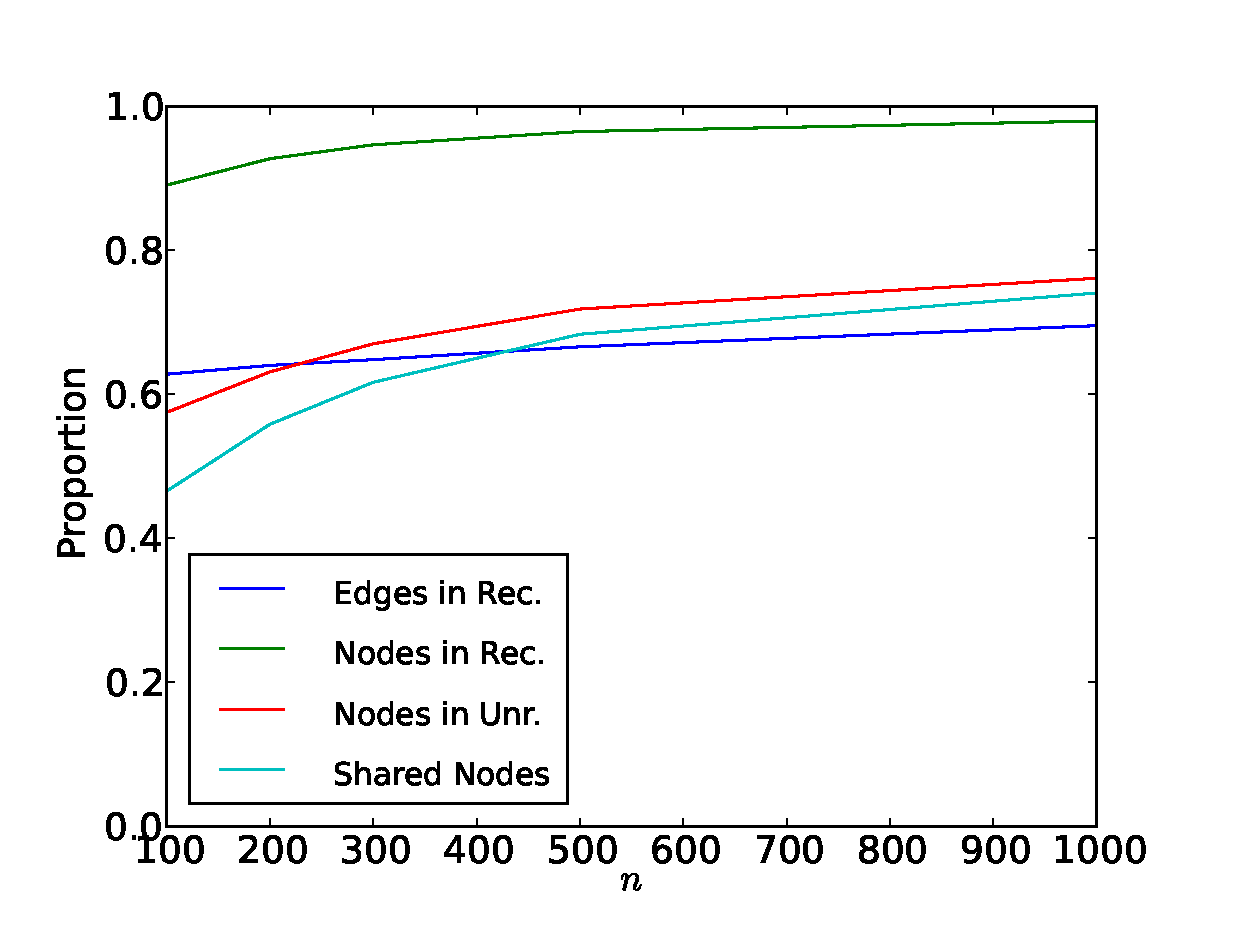
\includegraphics[width=1.5in]{proportion_edgesnodes_n}}                
\subfloat[Varying $k$]{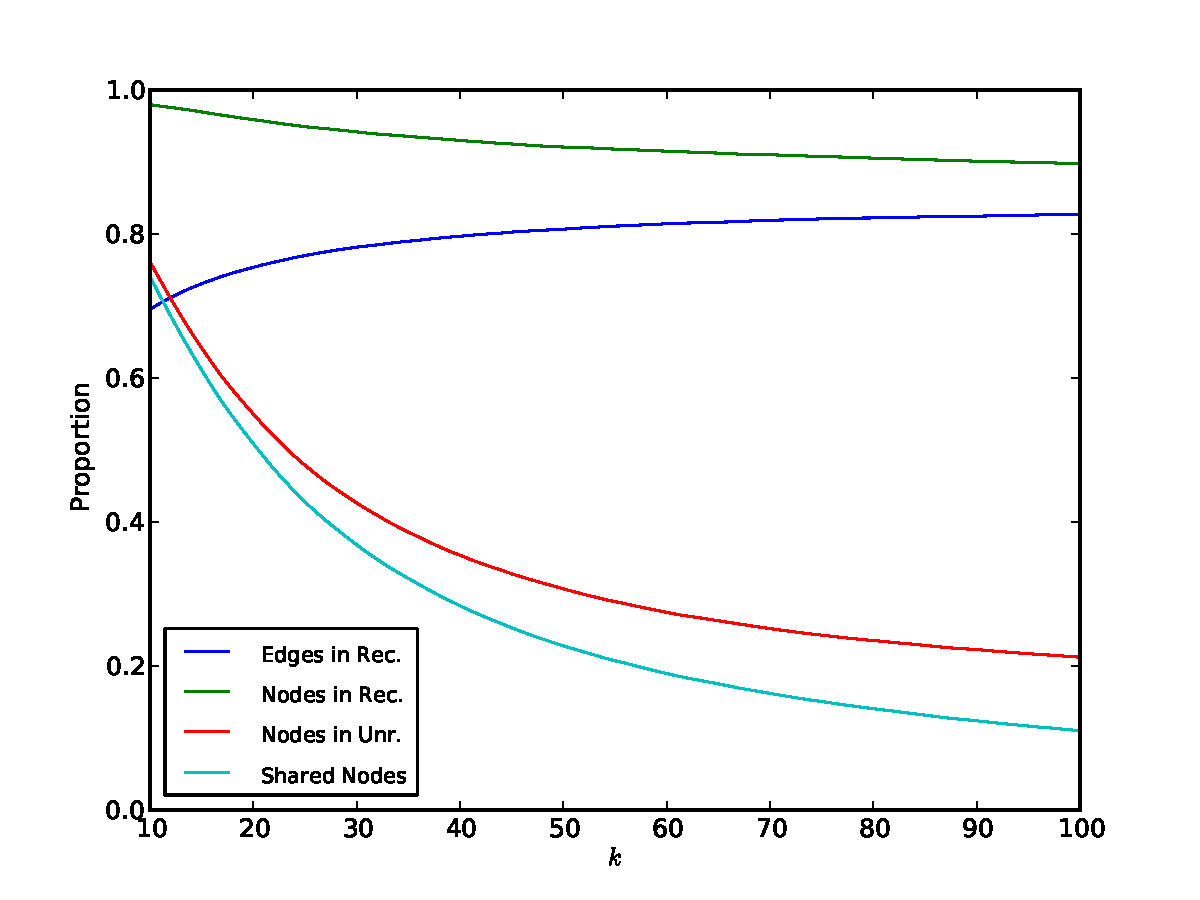
\includegraphics[width=1.5in]{proportion_edgesnodes_k}}
\caption{Proportion of nodes or edges}
\label{fig_rur_propne}
\end{figure}

\begin{figure}[!t]
\centering
\subfloat[Varying $n$]{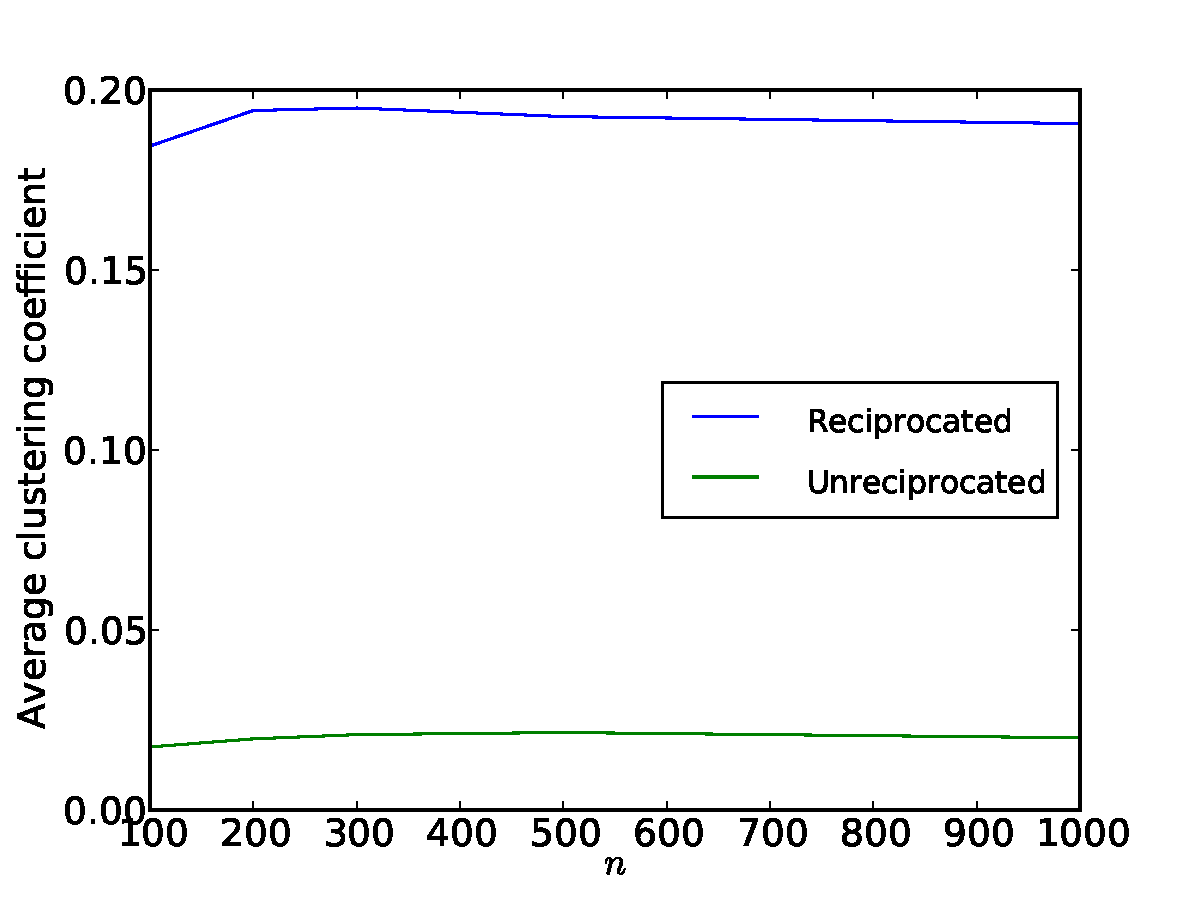
\includegraphics[width=1.5in]{average_clustering_n}}                
\subfloat[Varying $k$]{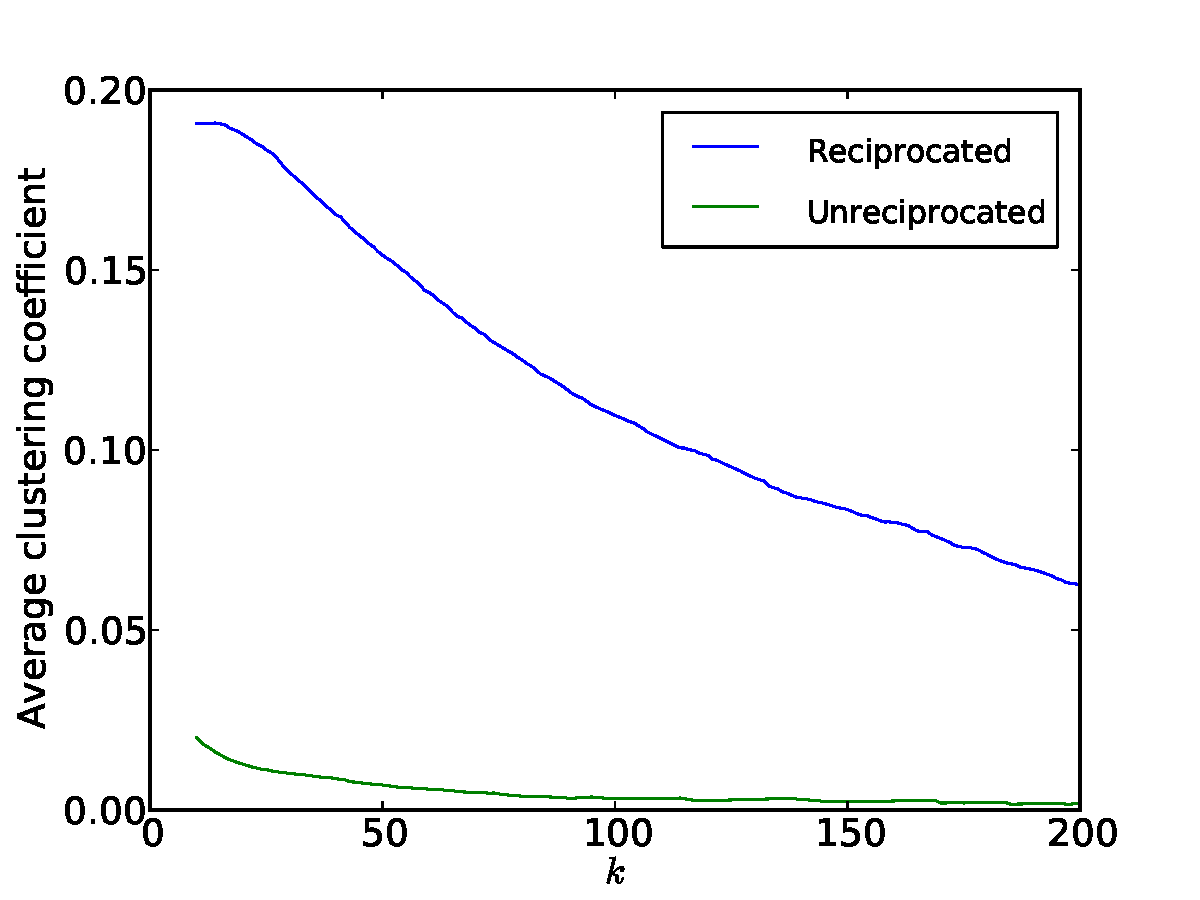
\includegraphics[width=1.5in]{average_clustering_k}}
\caption{Clustering coefficient}
\label{fig_rur_cc}
\end{figure}

\begin{figure}[!t]
\centering
\subfloat[Varying $n$]{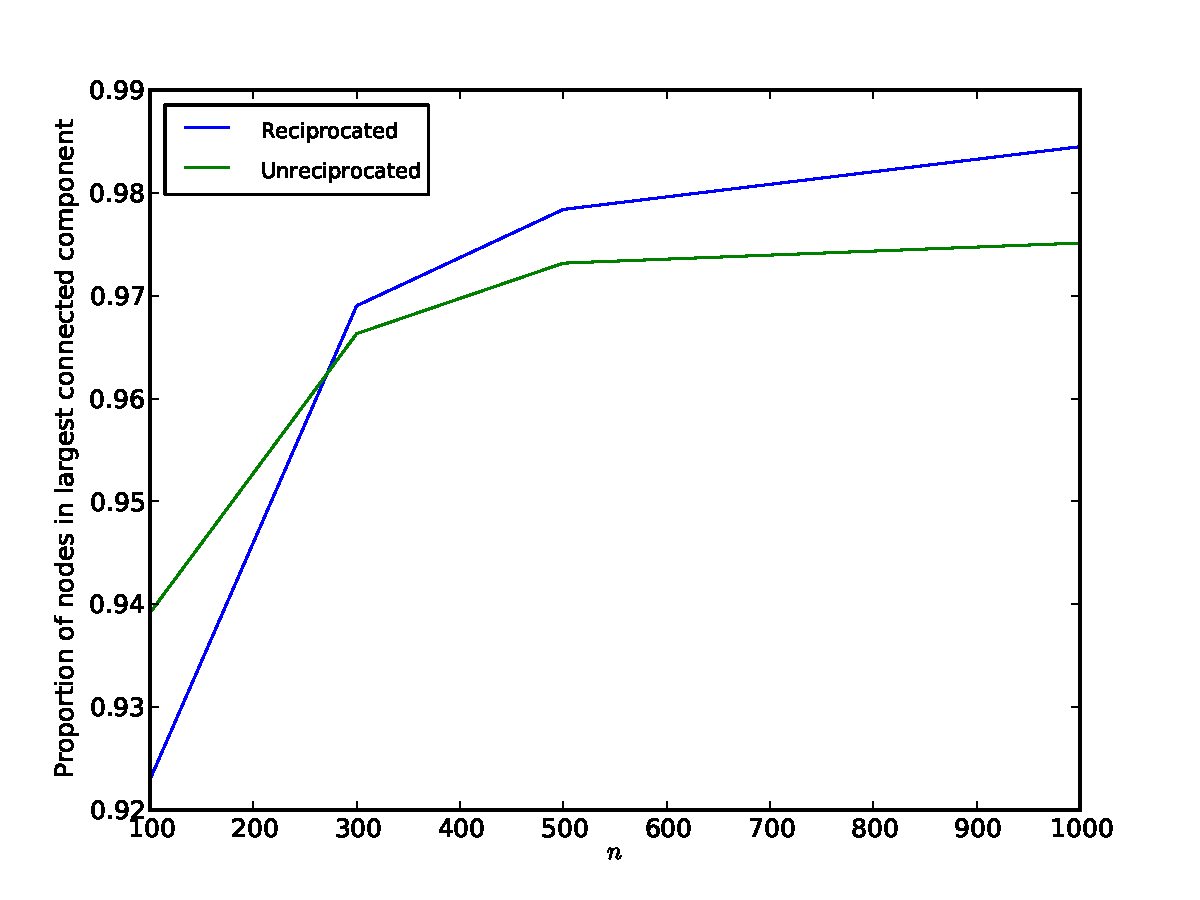
\includegraphics[width=1.5in]{proportion_largestcc_n}}                
\subfloat[Varying $k$]{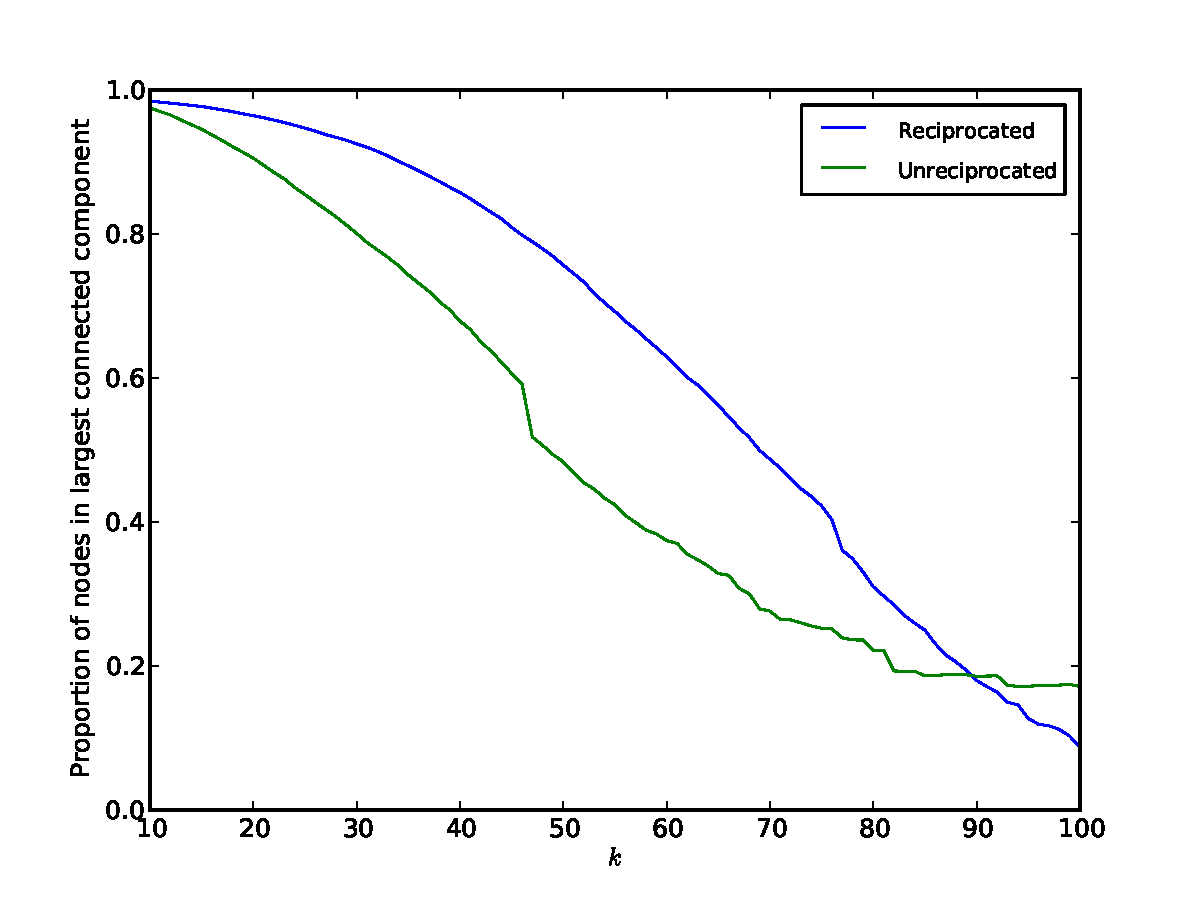
\includegraphics[width=1.5in]{proportion_largestcc_k}}
\caption{Proportion in largest connected component}
\label{fig_rur_lcc}
\end{figure}

\begin{figure}[!t]
\centering
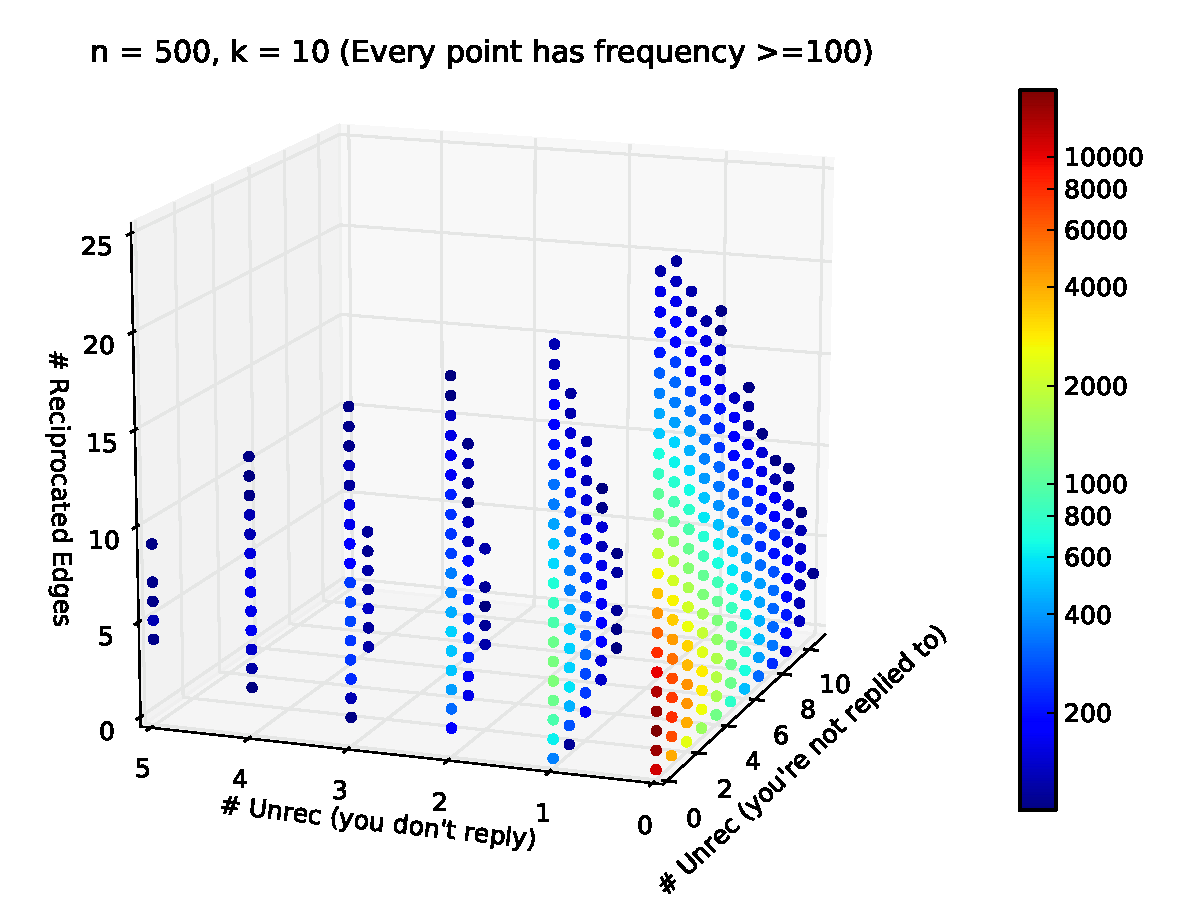
\includegraphics[width=2.5in]{scatter3}
\caption{Scatter plot of users' interaction types}
\label{fig_rur_sca2}
\end{figure}

% An example of a double column floating figure using two subfigures.
% (The subfig.sty package must be loaded for this to work.)
% The subfigure \label commands are set within each subfloat command, the
% \label for the overall figure must come after \caption.
% \hfil must be used as a separator to get equal spacing.
% The subfigure.sty package works much the same way, except \subfigure is
% used instead of \subfloat.
%
%\begin{figure*}[!t]
%\centerline{\subfloat[Case I]\includegraphics[width=2.5in]{subfigcase1}%
%\label{fig_first_case}}
%\hfil
%\subfloat[Case II]{\includegraphics[width=2.5in]{subfigcase2}%
%\label{fig_second_case}}}
%\caption{Simulation results}
%\label{fig_sim}
%\end{figure*}
%
% Note that often IEEE papers with subfigures do not employ subfigure
% captions (using the optional argument to \subfloat), but instead will
% reference/describe all of them (a), (b), etc., within the main caption.

\section{Conclusion}
To be written.


\section*{Acknowledgment}
The authors would like to thank Twitter for providing our experimental dataset. This work was supported by (SOMEGRANT).


\bibliographystyle{IEEEtran}
\bibliography{rec}

\end{document}


